%this is template for my % Template for INT1414 reports
%% by Thanh Le
%% based on LaTeX work of Robin Turner.
%% Adapted from the IEEE peer review template

%
% note that the "draftcls" or "draftclsnofoot", not "draft", option
% should be used if it is desired that the figures are to be displayed in
% draft mode.

\documentclass[conference]{IEEEtran}
\IEEEoverridecommandlockouts
\usepackage{cite} % Tidies up citation numbers.
\usepackage{url} % Provides better formatting of URLs.
\usepackage{booktabs} % Allows the use of \toprule, \midrule and \bottomrule in tables for horizontal lines
\usepackage{graphicx}

\usepackage{listings}


\hyphenation{op-tical net-works semi-conduc-tor} % Corrects some bad hyphenation 

% The preceding line is only needed to identify funding in the first footnote. If that is unneeded, please comment it out.
\usepackage{amsmath,amssymb,amsfonts}
\usepackage{algorithmic}
\usepackage{textcomp}
\usepackage{xcolor}
\def\BibTeX{{\rm B\kern-.05em{\sc i\kern-.025em b}\kern-.08em
    T\kern-.1667em\lower.7ex\hbox{E}\kern-.125emX}}


\begin{document}
\title{Deployment and Analysis of a Distributed PostgreSQL Database System Using the Pagila Dataset}

\author{\IEEEauthorblockN{Huynh Minh Thinh}
\IEEEauthorblockA{\textit{Department of Information Technology 2} \\
\textit{Posts and Telecommunications Institute of Technology at HCM city}\\
Ho Chi Minh City, Vietnam \\
D22CQCN01-N \\
n22dccn082@student.ptithcm.edu.vn}}
\date{}

\maketitle

% \IEEEpeerreviewmaketitle
\begin{abstract}
The abstract does not only mention the paper, but is the original paper shrunken to approximately 200 words. It states the purpose, reports the information obtained, gives conclusions, and recommendations. In short, it summarizes the main points of the study adequately and accurately. It provides information from every major section in the body of the report in a dense and compact way. Past tense and active voice is appropriate when describing what was done. If there is any, it includes key statistical detail.  

Depending on the format you use, the abstract may come on the title page or at the beginning of the main report.

\end{abstract}





\section{Introduction}

In today's digital world, a single database can struggle to keep up with the demands of a successful application. As more users connect and more data is collected, a traditional database can become a bottleneck, slowing everything down or even crashing entirely. Worse, if that single server fails, everything can be lost. A popular and effective solution to this problem is to move away from a single database and instead use a "distributed" system that spreads the work across multiple computers.

This project puts that solution into practice. I set out to build and analyze a small network—or cluster—of four PostgreSQL databases working together. Using PostgreSQL's own streaming replication feature, I configured one main "primary" server and three "hot-standby" replicas. This kind of setup is an industry standard for making sure a system stays online (high availability) and can handle many users reading data at once (read scalability). To test the cluster with realistic information, I loaded it with the Pagila sample dataset, which is designed to look like the database for a video rental store.

This report will walk you through the entire project. It starts by explaining the core problem of scaling a database and how replication helps solve it. I'll then cover the step-by-step process of setting up the virtual machines, configuring the main server and its replicas, and loading the Pagila data. After that, I will analyze how well this setup would support a busy web application, and I'll finish by summarizing what I learned and suggesting ideas for the future.
\section{Problem Definition}
Any successful website eventually hits two walls. The first is the "too popular" problem: so many people are using the site at once that it slows to a crawl. The second is the "everything is broken" problem: a single server fails, and the entire site goes offline.

For an online movie rental service, the "too popular" issue comes from having thousands of users Browse the catalog simultaneously. Most of what they do—searching for films, reading descriptions, checking actor pages—are read operations. These requests quickly overwhelm a single database server, leading to frustratingly slow load times for everyone.

The "everything is broken" problem is even more severe. If our one and only database server crashes, there is no backup. The entire service becomes unavailable, losing customers and revenue. This project's goal is to build a database system that solves both these problems: one that can handle a massive read workload without slowing down, and one that can survive a server failure without shutting down completely.

\section{Proposed Solutions}

With the main goals of speed and reliability in mind for a future large-scale site, I had to make a big decision right at the start: how should the data be organized across multiple servers? It really boiled down to two main philosophies: splitting the data up, or making copies of it.


\subsection{The "Divide and Conquer" Method: Sharding}
The first philosophy, sharding, is like deciding to replace one massive, central filing cabinet with several smaller ones. You'd organize them by a clear rule—for example, putting all customer files for names A-M in the first cabinet, and N-Z in the second.

The big advantage here is that you can have multiple people filing new documents at the same time, which is fantastic for handling a huge volume of new data (writes). The real challenge, though, is the new complexity. Your application now has to act like a smart receptionist, knowing exactly which cabinet to send someone to for a specific file. Any task that needs information from both cabinets, like a company-wide report, becomes a real puzzle to solve.

\subsection{The "Make a Copy" Method: Replication (My Chosen Solution)}
The other philosophy, and the one I chose for this project, is replication. Instead of splitting up the filing cabinet, I decided to keep the original as the one "master" source of truth, and then create several perfect duplicates.

The system operates on a simple rule: any new information (a write) must go to the master cabinet first. Once it's there, an identical copy of the update is immediately sent out to all the duplicate cabinets. The payoff for this is huge. When a hundred people need to look something up (a read), they can be sent to any of the available copies. This keeps the line at the master cabinet short, leaving it free to handle new, incoming information.


\section{Criteria for Assessing Solutions} \label{sec:criteria}
This may be a modified version of your proposal depending on previously carried out research or any feedback received.  



\section{Implementation Methodology}

\subsection{System Environment and Network Configuration}
% I built my four-node cluster using a mix of my main computer and some virtual ones. My physical machine was the primary server, and I ran the three standby servers as virtual machines (VMs) right on that same computer.
%
% To do this, I used KVM/QEMU for the virtualization part, mostly because it’s already built into Linux and works well. The virt-manager program was what I used to handle the VMs.
%
% To get all these servers talking to each other, I put them all on their own private network (192.168.122.0/24). This kept the important database traffic separate from everything else. A crucial step was giving each server a static IP address. I did this so the standby servers would never lose track of where the primary server was, which is essential for replication to work without issues.
%
% All the specific details, like the IP addresses I used for each server, are listed in Table \ref{tab:node_config}.

I built my four-node cluster using a mix of my main computer and some virtual ones. My physical machine was the primary server, and I ran the three standby servers as virtual machines (VMs) right on that same computer. To do this, I used KVM/QEMU for the virtualization part, managed with the `virt-manager` program.

To get all these servers talking to each other, I put them all on their own private network (`192.168.122.0/24`). This kept the important database traffic separate from everything else. A crucial step was giving each server a static IP address, which is essential for stable replication. The overall architecture is illustrated in Figure \ref{fig:architecture}, and the specific node details are listed in Table \ref{tab:node_config}.

\begin{figure}[!h]
    \centering
    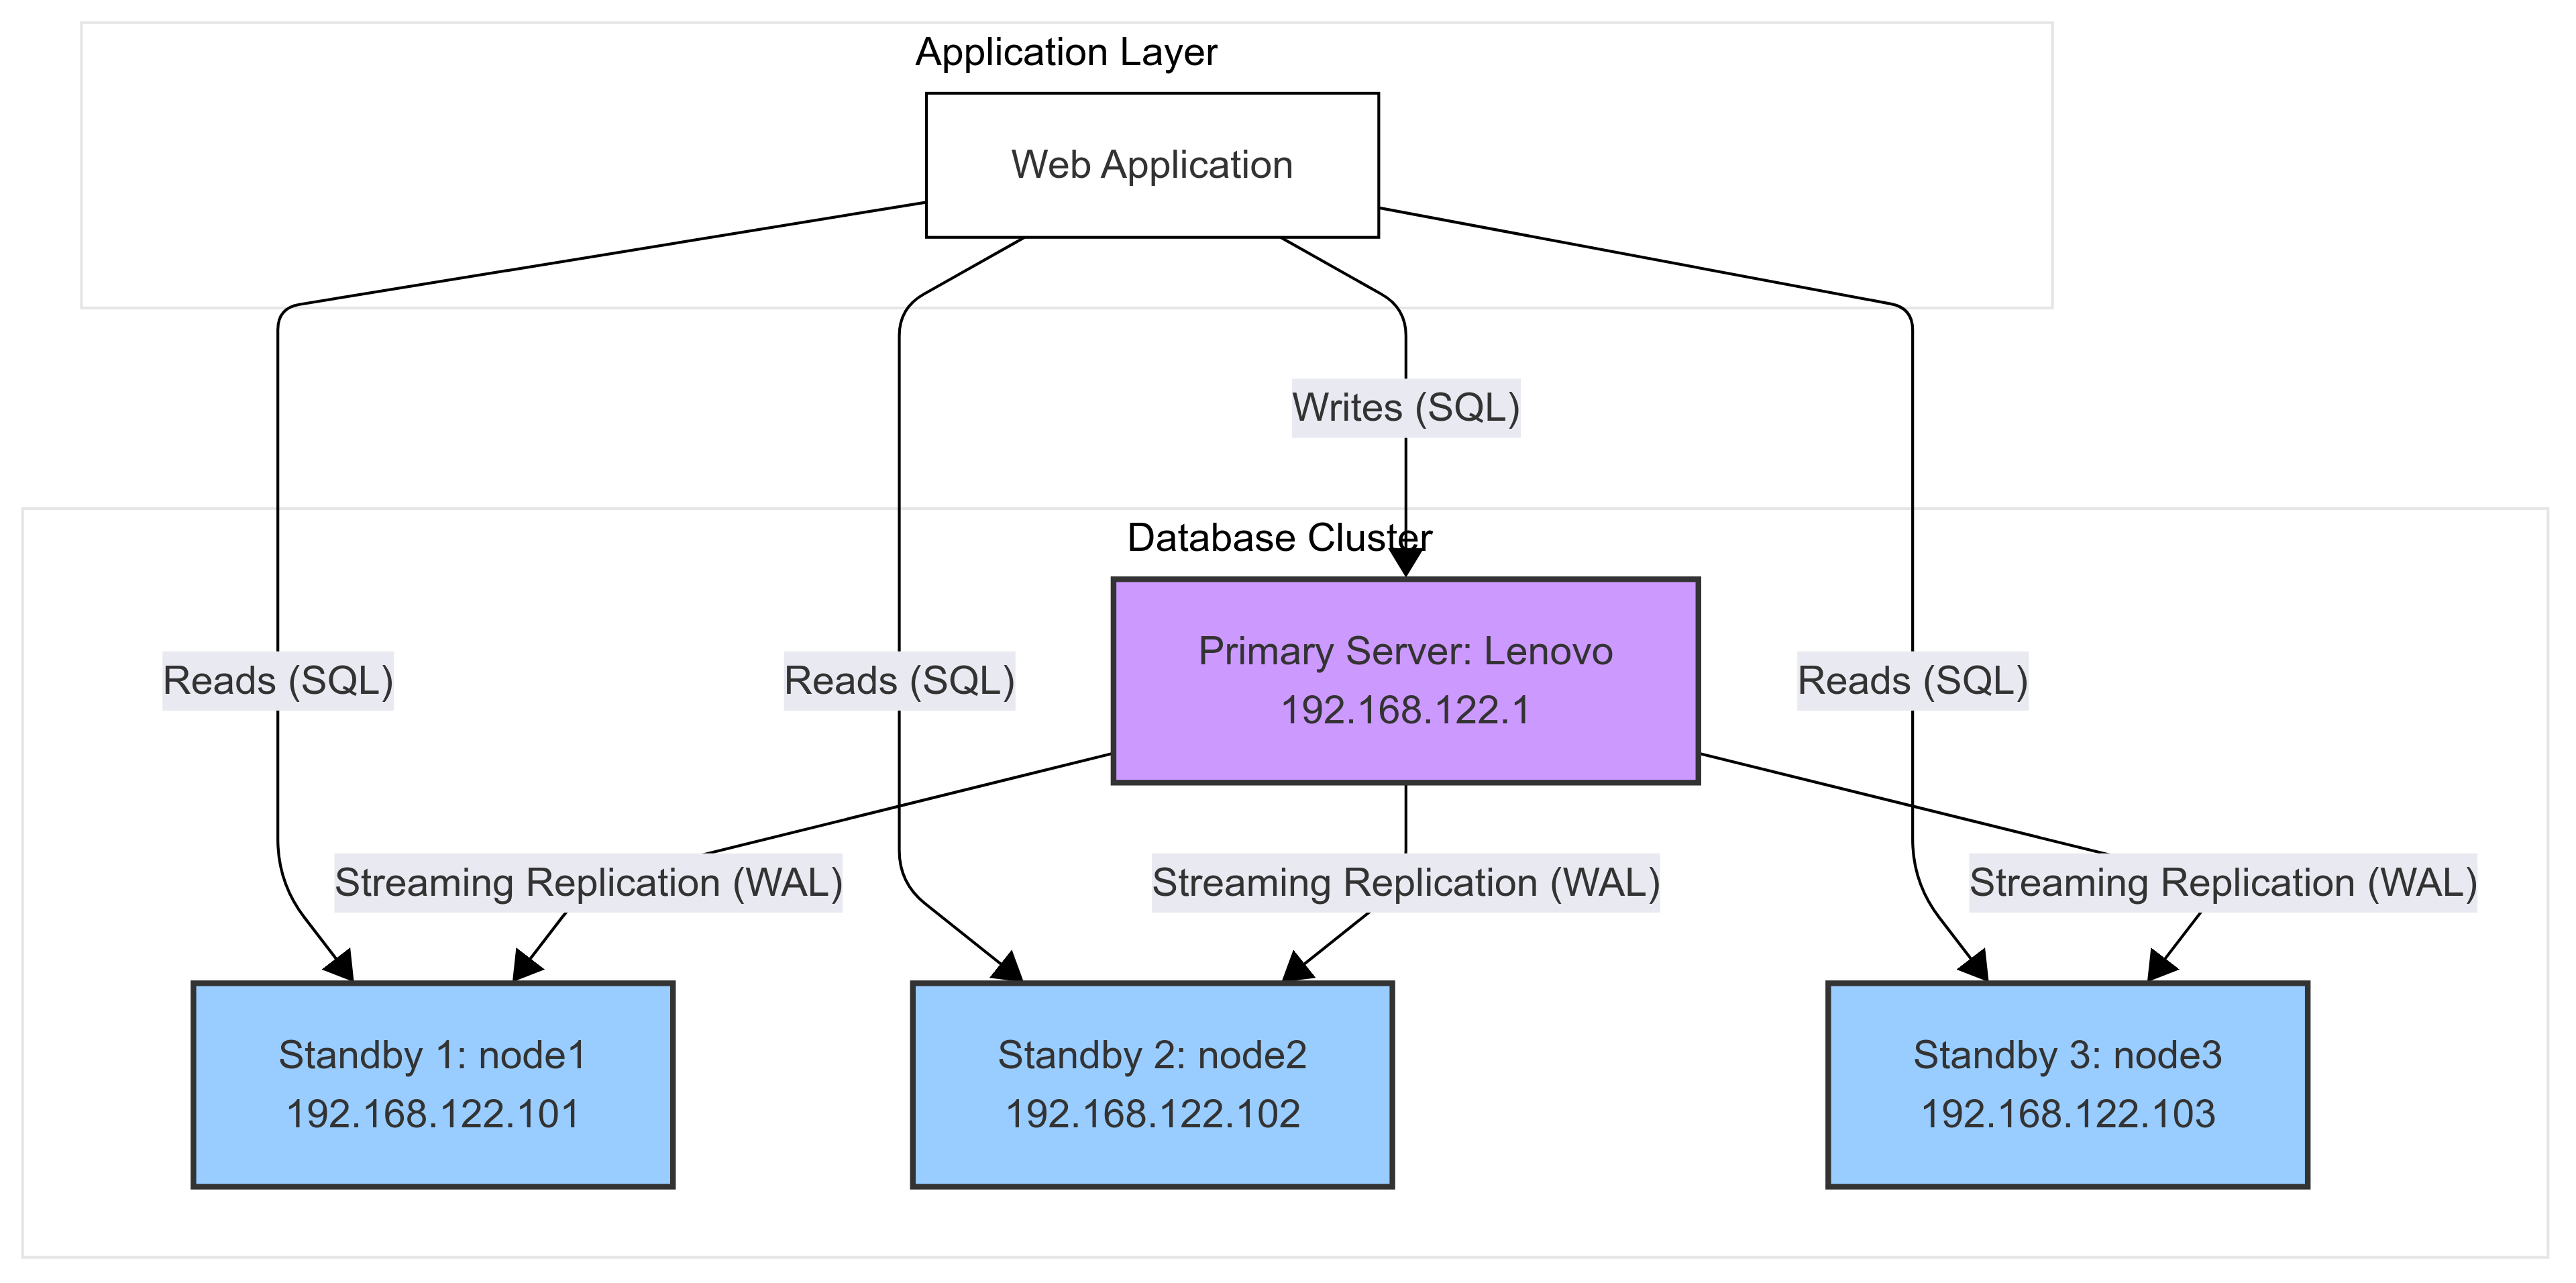
\includegraphics[width=0.9\columnwidth]{./images/architecture-diagram.png}
    \caption{The high-level architecture of the four-node replicated PostgreSQL cluster, showing the flow of write/read queries and the WAL replication stream.}
    \label{fig:architecture}
\end{figure}

\begin{table}[h!]
\centering
\caption{Node Configuration for the Distributed Cluster}
\label{tab:node_config}
\begin{tabular}{l l l l}
\toprule
\textbf{Role} & \textbf{Hostname} & \textbf{Operating System} & \textbf{Static IP Address} \\
\midrule
Primary   & Lenovo & EndeavourOS (Host) & 192.168.122.1 \\
Standby 1 & node1             & Ubuntu Server 24.04  & 192.168.122.101 \\
Standby 2 & node2             & Ubuntu Server 24.04  & 192.168.122.102 \\
Standby 3 & node3             & Ubuntu Server 24.04  & 192.168.122.103 \\
\bottomrule
\end{tabular}
\end{table}

\subsection{Standby Node Preparation}
To save time and make sure all the servers were identical, I didn't build each of the three standby nodes from scratch. Instead, I made a reusable template, which some people call a "golden image."

My starting point for the template was a clean installation of Ubuntu Server 24.04. I got it fully updated and then installed the essential software. The most important piece, naturally, was PostgreSQL version 17—it had to be an exact match to the primary server. I also threw in a couple of basic networking tools like openssh-server and iputils-ping to make life easier later on.

Once the template was good to go, I simply cloned it three times to create my three standby servers. This left me with three identical VMs, which was a great start, but they each needed their own unique identity before they could work together in the cluster. This meant making a few unique tweaks to each one:



\begin{enumerate}
\item \textbf{Gave it a new name:} I changed the hostname of each server using the hostnamectl command so I could tell them apart. For example, this is how I set the name for the first standby:
\begin{lstlisting}[language=bash, caption={Setting the hostname for node1}]
sudo hostnamectl set-hostname node1
\end{lstlisting}

\item \textbf{Set its IP address:} Next, I edited the Netplan configuration file (found in `/etc/netplan/`) to give each server its own static IP.

\item \textbf{Checked the connection:} Finally, I did a quick network check. I used the `ping` command from each server to make sure it could reach all the other nodes in the cluster, especially the primary.

\end{enumerate}

The very last thing I did on each standby server was to stop the PostgreSQL service from running with sudo systemctl stop postgresql. This was important because their data folders needed to be empty and ready for the next big step: copying all the data over from the primary server using the pg\_basebackup tool.


\subsection{Setting Up the Replication}
With the three standby servers prepped and waiting, the next step was to configure the primary server (Lenovo) to allow them to connect and then to actually create the replicas. This process felt a bit like setting up a secure radio broadcast: first, I had to turn on the transmitter on the primary, and then I had to give each standby a radio tuned to the right frequency.

First, I edited two core configuration files on the primary server. In postgresql.conf, I changed the listen\_addresses to ensure the server was listening for network connections, not just local ones. I also set wal\_level = replica, which tells PostgreSQL to write down enough information in its logs to allow a standby to perfectly reconstruct the data.

Next, in the pg\_hba.conf file—which acts as PostgreSQL's own firewall—I added a new rule. This rule explicitly gave a special user named replicator permission to connect from any of my standby servers for the purpose of replication.

With the primary server ready to broadcast its changes, it was time for the magic step: cloning the data. On each standby server, I ran the pg\_basebackup command. This powerful tool connects to the primary, makes a perfect binary copy of the entire database, and—thanks to the -R flag—automatically creates the necessary configuration files on the standby to tell it how to follow the primary.

sudo -u postgres pg\_basebackup -h Lenovo \
-U replicator -D /var/lib/postgresql/17/main \
-P -R -Xs

After the backup was complete on each standby, the final step was to simply start the PostgreSQL service. Upon starting, each standby read its new configuration, connected back to the Lenovo primary, and immediately began receiving a live stream of any new data changes. A quick check on the primary using SELECT * FROM pg\_stat\_replication; confirmed the result: all three standby nodes were connected and streaming, and my distributed cluster was officially online.


% The main difference between this section and the one in your report proposal is use of verb tense: there you suggested what you will do and here you will describe what you did. Be concise and precise when outlining how you researched your potential solutions. 
% Remember that your research should be guided by: 
% \begin{itemize}
% \item Relevance to the context of application  
% \item Your assessment criteria 
% \item Practicality 
% \end{itemize}
% So it may be worth commenting on your research methodology in light of the above (e.g., justifying a particular approach).  
%
% In this section, only describe how you collected data, and explain what you did to test your criteria.  \emph{Do not include your findings in this section.}

\section{Analysis and Interpretation}
%  In this section you will mainly analyze your data in terms of your assessment criteria; e.g., do the data suggest that a particular solution is ``cost effective'' ``environmentally acceptable'', ``technically feasible'' or ``affordable''?
%
% Be logical and selective when analyzing/interpreting your research data.  For example, if a proposed solution is proven to be far too expensive to realistically implement in your context, is there any value in discussing whether it is ``culturally viable'' or ``technically sustainable''? Perhaps in this case you can focus more attention on solutions that your research suggests are more valid.  Do not just throw huge quantities of raw data at your reader and leave them to interpret it. Present enough to transparently support any conclusions you draw and make sure that you offer justifications for your analysis.  
%
% Be honest and reflective while discussing your data. Your data might be too limited or unclear to interpret with accuracy---explain this, perhaps suggesting how this shortcoming could be addressed. Admitting the above will help you draw more honest and worthwhile conclusions.  
%
% Remember that research is an imperfect and ongoing process that should be open to question and verification. Therefore, unless convinced by the absolute strength of your evidence, you should be tentative in your language choice when interpreting/analyzing research results. Selectively use {\em hedging} (language which indicates a lack of certainty) to modify the tone of your analysis and any conclusions that result from this. 
%
% Here are some examples that show differing degrees of certainty:
% \begin{itemize}  
% \item it appears that \ldots
% \item it can be tentatively concluded that \ldots
% \item it is almost certain that \ldots
% \item perhaps the evidence indicates \ldots
% \item this seems to point to the fact that \ldots
% \item this could be interpreted as evidence of \ldots
% \item without doubt its application would prove beneficial for \ldots
% \end{itemize}
%
% Finally, don’t introduce any new content (e.g., research methods or solutions) within this section---this will prove confusing for the reader. The reader should clearly understand that you are, based on specific criteria, interpreting the results of your research in order to test the viability of various solutions to remedy a particular problem. The sole function of this part of the report is to openly discuss your research findings in order to set up your conclusions/recommendations.
%

% Example of a table from http://www.latextemplates.com/template/professional-table
\begin{table} % Add the following just after the closing bracket on this line to specify a position for the table on the page: [h], [t], [b] or [p] - these mean: here, top, bottom and on a separate page, respectively
\centering % Centers the table on the page, comment out to left-justify
\begin{tabular}{l c c c c c} % The final bracket specifies the number of columns in the table along with left and right borders which are specified using vertical bars (|); each column can be left, right or center-justified using l, r or c. To specify a precise width, use p{width}, e.g. p{5cm}
\toprule % Top horizontal line
& \multicolumn{5}{c}{Growth Media} \\ % Amalgamating several columns into one cell is done using the \multicolumn command as seen on this line
\cmidrule(l){2-6} % Horizontal line spanning less than the full width of the table - you can add (r) or (l) just before the opening curly bracket to shorten the rule on the left or right side
Strain & 1 & 2 & 3 & 4 & 5\\ % Column names row
\midrule % In-table horizontal line
GDS1002 & 0.962 & 0.821 & 0.356 & 0.682 & 0.801\\ % Content row 1
NWN652 & 0.981 & 0.891 & 0.527 & 0.574 & 0.984\\ % Content row 2
PPD234 & 0.915 & 0.936 & 0.491 & 0.276 & 0.965\\ % Content row 3
JSB126 & 0.828 & 0.827 & 0.528 & 0.518 & 0.926\\ % Content row 4
JSB724 & 0.916 & 0.933 & 0.482 & 0.644 & 0.937\\ % Content row 5
\midrule % In-table horizontal line
\midrule % In-table horizontal line
Average Rate & 0.920 & 0.882 & 0.477 & 0.539 & 0.923\\ % Summary/total row
\bottomrule % Bottom horizontal line
\end{tabular}
\smallskip 
\caption{Some impressive numbers} % Table caption, can be commented out if no caption is required
\label{tab:template} % A label for referencing this table elsewhere, references are used in text as \ref{label}
\end{table}
A reference to Table \ref{tab:template}.

\section{Conclusions and Recommendations}
Conclusion shows what knowledge comes out of the report. As you draw a conclusion, you need to explain it in terms of the preceding discussion. You are expected to repeat the most important ideas you have presented, without copying. Adding a table/chart summarizing the results of your findings might be helpful for the reader to clearly see the most optimum solution(s). 

It is likely that you will briefly describe the comparative effectiveness and suitability of your proposed solutions. Your description will logically recycle language used in your assessing criteria (section \ref{sec:criteria}): ``Solution A proved to be the most cost effective of the alternatives'' or ``Solution B, though a viable option in other contexts, was shown to lack adaptability''.  Do not have detailed analysis or lengthy discussions in this section, as this should have been completed in section X. 
 
As for recommendations, you need to explain what actions the report calls for. These recommendations should be honest, logical and practical. You may suggest that one, a combination, all or none of your proposed solutions should be implemented in order to address your specific problem. You could also urge others to research the issue further, propose a plan of action or simply admit that the problem is either insoluble or has a low priority in its present state.   

The recommendations should be clearly connected to the results of the report, and they should be explicitly presented. Your audience should not have to guess at what you intend to say.  




\appendices
\section{What Goes in the Appendices} \label{App:WhatGoes}
The appendix is for material that readers only need to know if they are studying the report in depth. Relevant charts, big tables of data, large maps, graphs, etc. that were part of the research, but would distract the flow of the report should be given in the Appendices. 
\section{Formatting the Appendices} \label{App:Formatting}
Each appendix needs to be given a letter (A, B, C, etc.) and a title. \LaTeX will do the lettering automatically.


% \begin{thebibliography}{1}
% Here are a few examples of different citations 
% Book
% \bibitem{kopka_1999} % Note the label in the curly brackets. Use the cite the source; e.g., \cite{kopka_latex}
% H.~Kopka and P.~W. Daly, \emph{A Guide to \LaTeX}, 3rd~ed.\hskip 1em plus
%   0.5em minus 0.4em\relax Harlow, England: Addison-Wesley, 1999.
% \bibitem{horowitz_2005}D.~Horowitz, \emph{End of Time}. New York, NY, USA: Encounter Books, 2005. [E-book] Available: ebrary, \url{http://site.ebrary.com/lib/sait/Doc?id=10080005}. Accessed on: Oct. 8, 2008.
% % Article from database
% \bibitem{castlevecchi_2008}D.~Castelvecchi, ``Nanoparticles Conspire with Free Radicals'' \emph{Science News}, vol.174, no. 6, p. 9, September 13, 2008. [Full Text]. Available: Proquest, \url{http://proquest.umi.com/pqdweb?index=52&did=1557231641&SrchMode=1&sid=3&Fmt=3&VInst=PROD&VType=PQD&RQT=309&VName=PQD&TS=1229451226&clientId=533}. Accessed on: Aug.~3, 2014.
% % Conference Paper from the Internet
% \bibitem{lach_2010}J.~Lach, ``SBFS: Steganography based file system,'' in \emph{Proceedings of the 2008 1st International Conference on Information Technology, IT 2008, 19-21 May 2008, Gdansk, Poland.} Available: IEEE Xplore, \url{http://www.ieee.org}. [Accessed: 10 Sept. 2010].
% % Web page, no author
% \bibitem{a_laymans_explanation}``A `layman's' explanation of Ultra Narrow Band technology,'' Oct.~3, 2003. [Online]. Available: \url{http://www.vmsk.org/Layman.pdf}. [Accessed: Dec.~3, 2003]. 
% \end{thebibliography}
%
% % This is a hand-made bibliography. If you want to use a BibTeX file, you're on your own ;-)
%
%
%
%
%
%
%
%
%
%
%
%
%
\end{document}


